Der Koeffizient $\alpha_t$ für den ausgewählen schwachen Lerner $h_t$ wird durch den minimalen Verlust berechnet. Daher wird dieser zunächst als
exponentieller Verlust definiert:
\begin{align*}
    L(h_t) = \sum_{i=1}^{m} w_i^{(t)}e^{-y_ih_t(x_i)}
\end{align*}
Der Lernkoeffizient $\alpha_t$ wird nun als Faktor im Exponenten eingeführt:
\begin{align*}
    L(h_t)=\sum_{i=1}^{m}w_i^{(t)}e^{-\alpha_ty_ih_t(x_i)}
\end{align*}
Korrekt und falsch vorhergesagte Daten haben nun je folgenden Einfluss auf den Verlust:
\begin{align*}
    y_i = h_t(x_i)    & \implies y_ih_t(x_i)  = 1                                     \\
                      & \leadsto \text{ Beitrag zum Verlust: } w_i^{(t)}e^{-\alpha_t} \\
    y_i \neq h_t(x_i) & \implies y_ih_t(x_i)  = -1                                    \\
                      & \leadsto \text{ Beitrag zum Verlust: } w_i^{(t)}e^{\alpha_t}
\end{align*}
So lässt sich der Verlust in je einen Teil für korrekt und falsch vorhergesagte Daten aufteilen:
\begin{align*}
    L(h_t) = \sum_{y_i=h_t(x_i)}w_i^{(t)}e^{-\alpha_t} + \sum_{y_i\neq h_t(x_i)} w_i^{(t)}e^{\alpha_t} \\
\end{align*}
Nun soll $\alpha_t$ so gewählt werden, dass der Fehler minimiert wird. Entprechend wird nach $\alpha_t$ abgeleitet und $L(h_t)'$=0 gesetzt:
\begin{align*}
    \frac{dL(h_t)}{d\alpha_t} & = -e^{-\alpha_t}\sum_{y_i=h_t(x_i)}w_i^{(t)} + e^{\alpha_t}\sum_{y_i\neq h_t(x_i)}w_i^{(t)} = 0                             \\
                              & \Leftrightarrow e^{2\alpha_t} = \frac{\sum_{y_i=h_t(x_i)}w_i^{(t)}}{\sum_{y_i\neq h_t(x_i)}w_i^{(t)}}                       \\
                              & \Leftrightarrow \alpha_t = \frac{1}{2}\ln\left(\frac{\sum_{y_i=h_t(x_i)}w_i^{(t)}}{\sum_{y_i\neq h_t(x_i)}w_i^{(t)}}\right)
\end{align*}
Da $\varepsilon_t=\sum_{h_t(x_i)\neq y_i}w_i^{(t)}$ ist und aus der Tatsache, dass die Summe der Gewichte 1 ist folgt, dass $1-\varepsilon_t=\sum_{h_t(x_i)= y_i}w_i^{(t)}$ lässt
sich $\alpha_t$ berechnen durch:
$$
    \alpha_t = \frac{1}{2}\ln\left(\frac{1-\varepsilon_t}{\varepsilon_t}\right)
$$
\begin{figure}
    \centering
    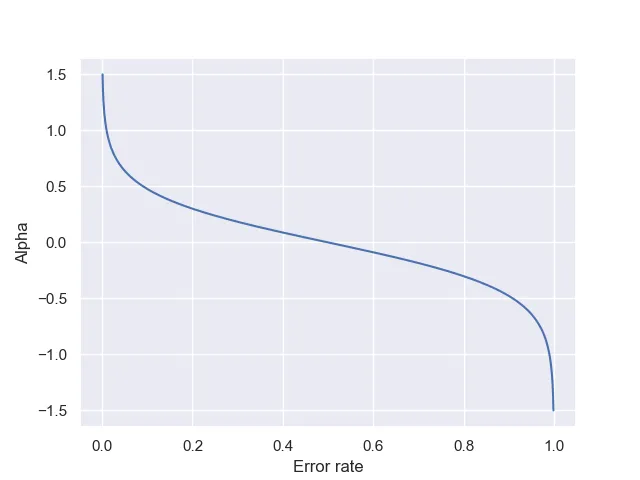
\includegraphics[width=0.5\textwidth]{figures/alpha_graph.png}
    \caption{Verhalten von $\alpha_t$ in Anhängigkeit von $\varepsilon_t$}
\end{figure}
Dieser gibt an, wie stark die Vorhersage dieses schwachen Lerners im späteren Ensemble
gewichtet wird und bestimmt die Aktualisierung der Gewichte für die nächste Iteration.